% Results section skeleton. Requires graphicx, booktabs, float.
% \fillin{} = still to fill in. Pi values: runs from 2026-10-25, prediction = window.

\providecommand{\fillin}[1]{\textbf{[#1]}}
\providecommand{\figplaceholder}[1]{%
  \fbox{\parbox[c][4.5cm][c]{0.92\linewidth}{\centering\small #1}}}

\section{Results}
\label{sec:results}

This section compares the kernel-offloaded implementation with the userspace
baseline. Four tests were devised to be run on each testbed, where both the kernel-offloaded implementation and the userspace baseline is evaluated under blocking and non-blocking workloads.


Section~\ref{sec:res-workload} describes the workload and the
evaluation coverage of each run. Sections~\ref{sec:res-loss}
and~\ref{sec:res-cpu} report how much traffic reached the detector and at
what CPU cost, and Section~\ref{sec:res-detection} the resulting detection
quality, all with blocking disabled. Section~\ref{sec:res-blocking} covers
blocking, Section~\ref{sec:res-other} memory and decision delay, and
Section~\ref{sec:res-summary} summarises the findings. Each subsection
reports the results from the Raspberry Pi 400 first and those from the
FABRIC VM second. All runs use XDP in generic mode, with one run per
configuration (Table~\ref{tab:runs}). Detection results use the per-window
verdict (\texttt{window}).

\begin{table}[H]
  \centering
  \small
  \begin{tabular}{llll}
    \toprule
    Testbed & Run ID & Implementation & Blocking \\
    \midrule
    Raspberry Pi 400 & \texttt{usr-acc-gen-1} & Userspace & Off \\
                     & \texttt{ker-acc-gen-1} & Kernel    & Off \\
                     & \texttt{usr-per-gen-1} & Userspace & On  \\
                     & \texttt{ker-per-gen-1} & Kernel    & On  \\
    \midrule
    FABRIC VM        & \texttt{usr-acc-gen-1} & Userspace & Off \\
                     & \texttt{ker-acc-gen-1} & Kernel & Off \\
                     & \texttt{usr-per-gen-1} & Userspace & On \\
                     & \texttt{ker-per-gen-1} & Kernel & On \\
    \bottomrule
  \end{tabular}
  \caption{Runs presented in this section.}
  \label{tab:runs}
\end{table}

% ---------------------------------------------------------------------
\subsection{Workload and Evaluation Coverage}
\label{sec:res-workload}

\begin{figure}[H]
  \centering
  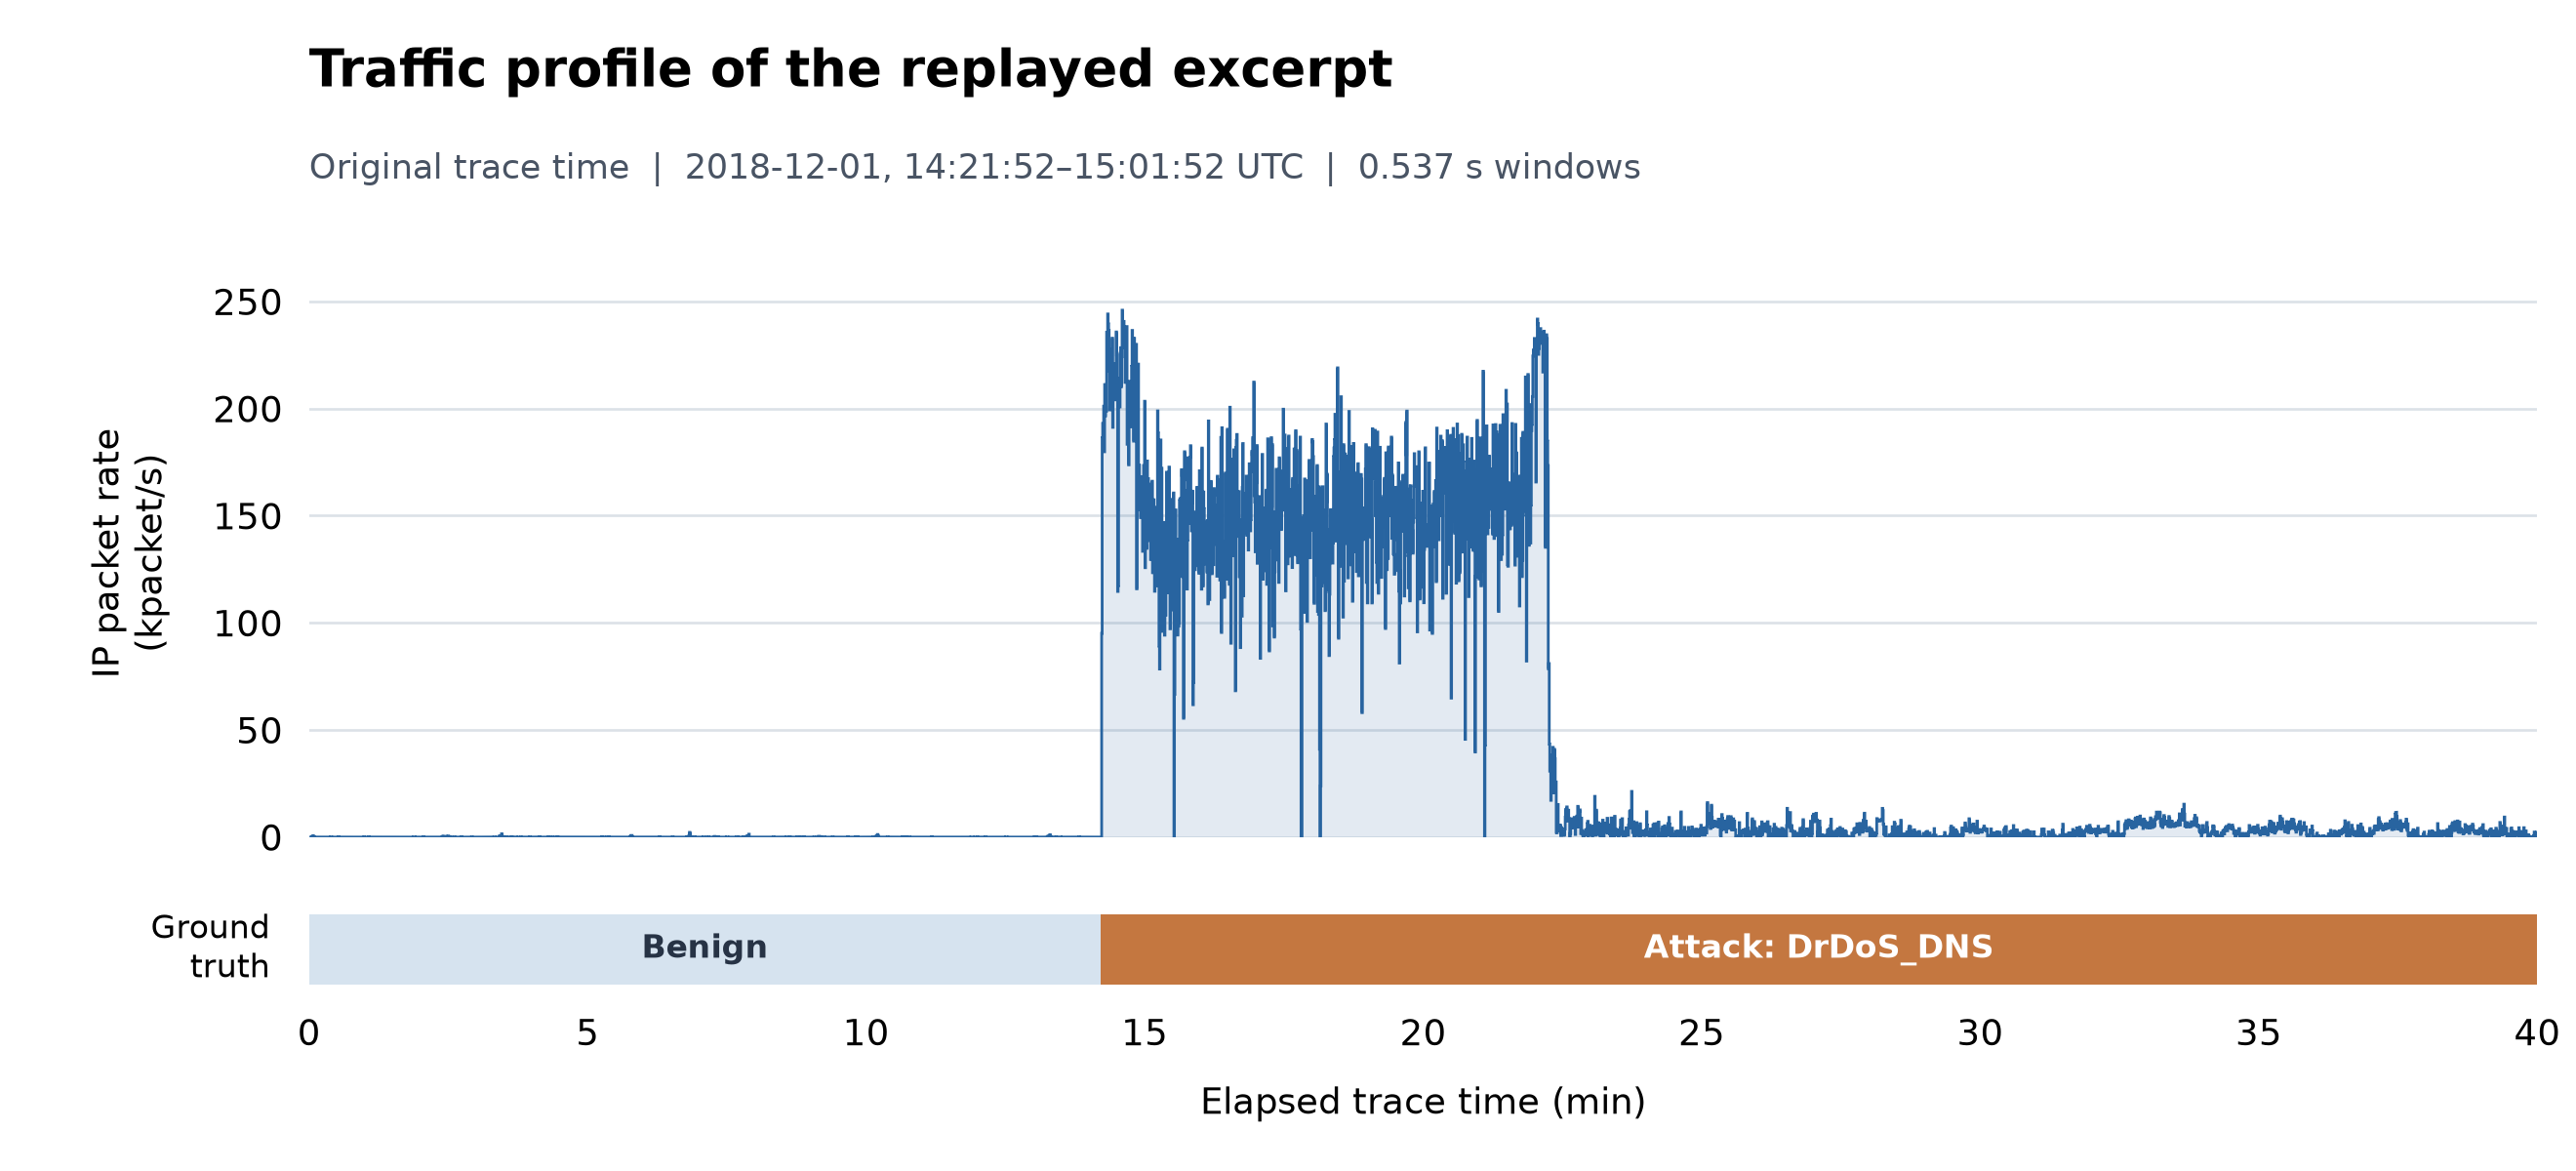
\includegraphics[width=\linewidth]{resources/testing-figures/figure-08-traffic-profile.png}
  \caption{Traffic profile of the replayed excerpt from saved offline PCAP-reference windows. Bottom: saved window-level ground truth from the corrected-label evaluation, using combined-window semantics.}
  \label{fig:workload}
\end{figure}

The excerpt contains 78,567,754 IP packets and one attack type, DrDoS\_DNS.
It consists of a benign period of approximately 14~minutes, a high-rate
flood of approximately 8~minutes, and a low-rate tail that is labelled as
attack until the end of the excerpt (Figure~\ref{fig:workload}).

Live windows are mapped to trace time by a single offset per run, found by
cross-correlating packets per window with an offline run of the excerpt.
To check this mapping independently of the detector's verdicts, the flood
onset was located in each run's own counted traffic, as the first window in
which the median packet count over nine consecutive windows exceeds 10,000.

\paragraph{Raspberry Pi 400}

\begin{table}[H]
  \centering
  \small
  \begin{tabular}{lrr}
    \toprule
    & \texttt{usr-acc-gen-1} & \texttt{ker-acc-gen-1} \\
    \midrule
    Windows closed               & 4,918 & 4,973 \\
    Excluded: before excerpt     & 0     & 94 \\
    Excluded: after excerpt      & 1,236 & 411 \\
    Excluded: warm-up            & 75    & 75 \\
    Excluded: not evaluated      & 1     & 0 \\
    Windows scored               & 3,606 & 4,393 \\
    \midrule
    Alignment correlation        & 0.589 & 0.684 \\
    Peak ratio to next candidate & 1.003 & 1.001 \\
    Flood onset vs.\ label start (s) & $-156.8$ & $+2.1$ \\
    Flood duration in counted traffic (s) & 771 & 672 \\
    \bottomrule
  \end{tabular}
  \caption{Evaluation coverage and alignment, Raspberry Pi 400, blocking
  disabled. The evaluator requires a correlation of at least 0.9 and a peak
  ratio of at least 1.2.}
  \label{tab:coverage}
\end{table}

Both Pi runs fail the evaluator's alignment criteria (Table~\ref{tab:coverage}).
For the kernel run, the flood onset falls 2.1~s after the labelled attack
start. For the userspace run, it falls 156.8~s before it, and the flood
lasts 99~s longer than in the kernel run. In the userspace run, the replay
had already been running for approximately 10 minutes when the
detector started, so its scored period begins later in the excerpt and
contains fewer benign windows.

\paragraph{FABRIC VM}

\begin{table}[H]
  \centering
  \small
  \begin{tabular}{@{}lrr@{}}
    \toprule
    & Userspace & Kernel \\
    \midrule
    Windows closed & 5,257 & 5,028 \\
    Excluded: before excerpt & 4 & 10 \\
    Excluded: after excerpt & 785 & 550 \\
    Excluded: warm-up & 75 & 75 \\
    Excluded: not evaluated & 0 & 0 \\
    Windows scored & 4,393 & 4,393 \\
    Alignment correlation & 0.744 & 0.738 \\
    Peak ratio to next candidate & 1.003 & 1.001 \\
    Flood onset vs.\ label start (s) & $-0.03$ & $-2.17$ \\
    Flood duration in counted traffic (s) & 726.9 & 729.1 \\
    \bottomrule
  \end{tabular}
  \caption{Evaluation coverage and alignment on the FABRIC VM, blocking disabled. Both runs use the saved evaluator alignment; no onset correction is applied.}
  \label{tab:fabric-coverage}
\end{table}

Both FABRIC evaluations score 4,393 windows, including 2,881 attack-labelled
and 1,512 benign-labelled windows (Table~\ref{tab:fabric-coverage}). Unlike
the Pi userspace evaluation, both cover the beginning of the excerpt.
The counted flood begins $-0.03$~s relative to the labelled attack start in
userspace and $-2.17$~s in the kernel run. However, both runs fail the evaluator's
correlation and peak-ratio criteria. Their flood durations are 726.9 and
729.1~s, compared with 489.1~s in the offline reference under the same
traffic-based rule. Matching the onset therefore does not validate the
remaining replay timeline.

For the FABRIC phase summaries, the median is centred over nine consecutive
windows. The first and last qualifying window starts are the cutpoints of
a half-open flood interval; boundary windows belong to exactly one phase.
Elapsed phase times are measured from the first recorded window, not process
launch. The runs also report different source commits and modified source
trees, so the implementation comparisons below are descriptive observations.


% ---------------------------------------------------------------------
\subsection{Packet Accounting and Loss}
\label{sec:res-loss}

\paragraph{Raspberry Pi 400}

\begin{figure}[H]
  \centering
  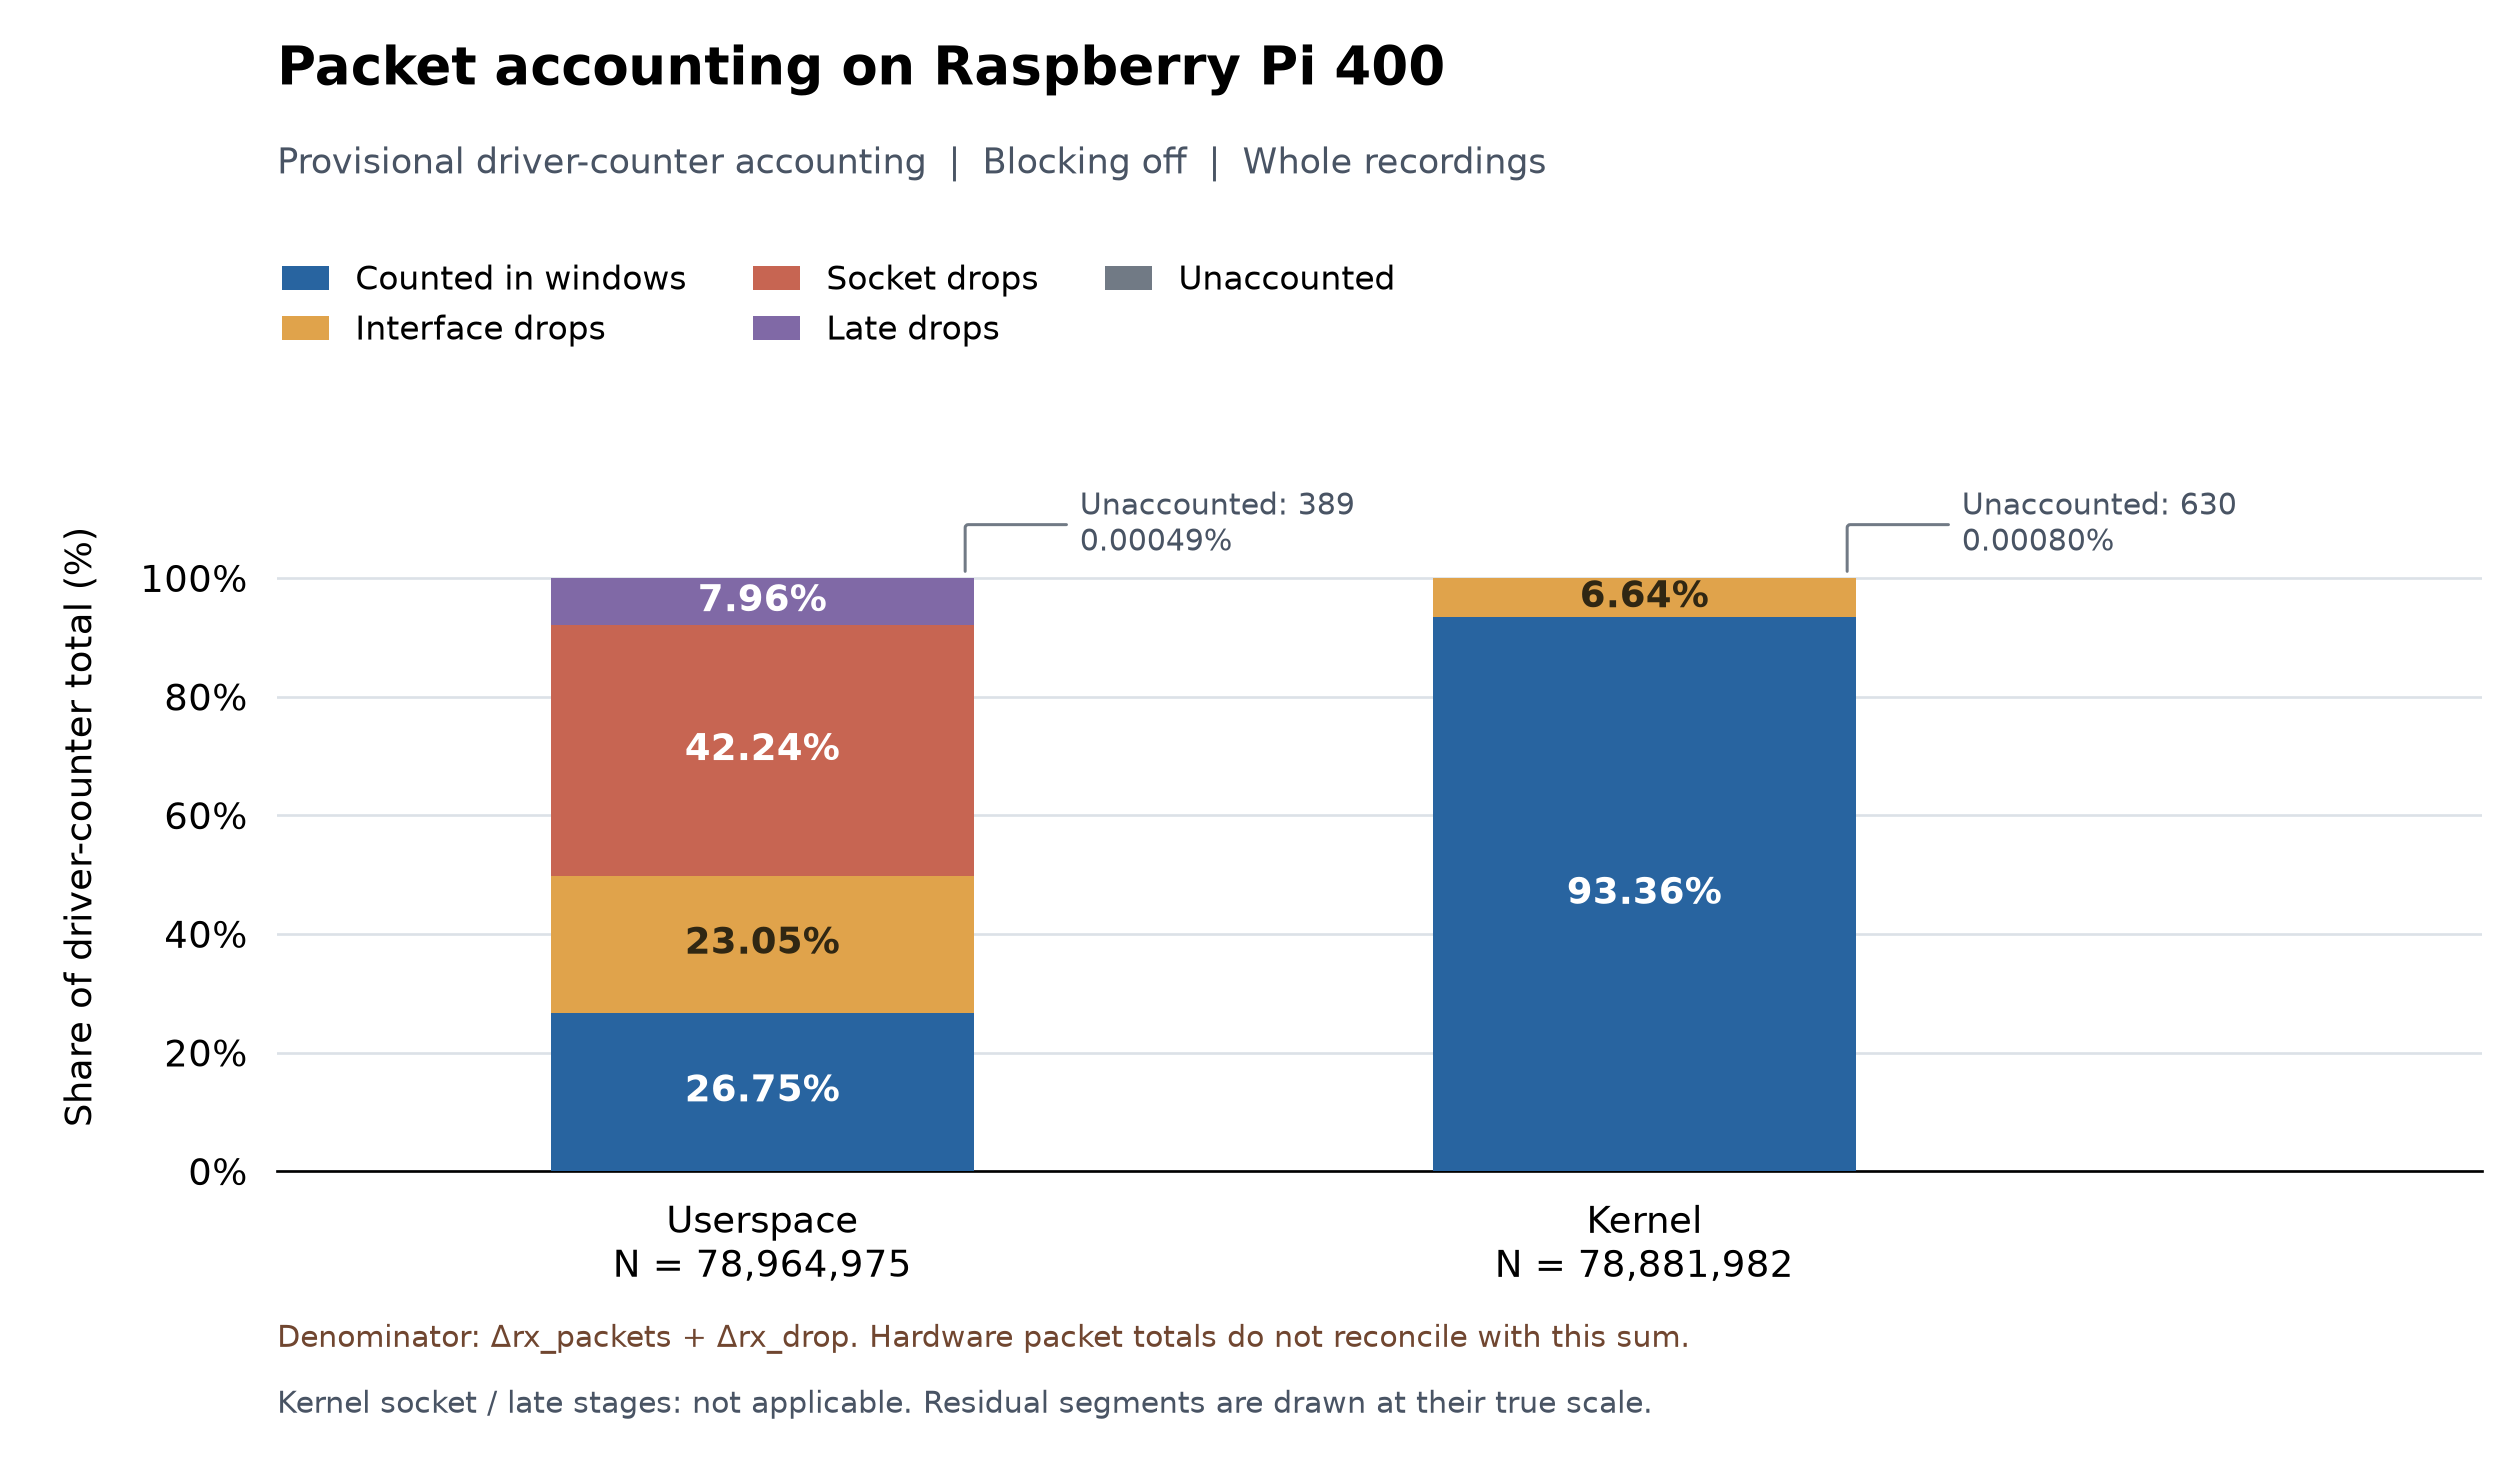
\includegraphics[width=\linewidth]{resources/testing-figures/figure-09-packet-accounting.png}
  \caption{Packet accounting on the Raspberry Pi 400 with blocking disabled,
  as a share of the packets seen by the interface.}
  \label{fig:loss}
\end{figure}

\begin{table}[H]
  \centering
  \small
  \begin{tabular}{lrrrr}
    \toprule
    & \multicolumn{2}{c}{Userspace} & \multicolumn{2}{c}{Kernel} \\
    \cmidrule(lr){2-3}\cmidrule(lr){4-5}
    & Packets & \% & Packets & \% \\
    \midrule
    Seen by interface & 78,964,975 & 100.00 & 78,881,982 & 100.00 \\
    \midrule
    Interface drops (\texttt{rx\_drop})        & 18,201,335 & 23.05 & 5,238,189  & 6.64 \\
    Capture-socket drops                       & 33,356,522 & 42.24 & --         & -- \\
    Late drops (window already closed)         & 6,283,426  & 7.96  & --         & -- \\
    Unaccounted                                & 389        & 0.00  & 630        & 0.00 \\
    Counted in windows                         & 21,123,303 & 26.75 & 73,643,163 & 93.36 \\
    \bottomrule
  \end{tabular}
  \caption{Packet accounting over the whole run with blocking disabled,
  Raspberry Pi 400. The denominator, \texttt{rx\_packets} + \texttt{rx\_drop},
  is an estimate based on the interface counters. The kernel implementation has no capture socket and no
  late-drop mechanism. For reference, the evaluator's window loss, measured
  against the 78,567,754 packets of the excerpt over the scored period, is
  73.4\% for userspace and 7.0\% for the kernel implementation.}
  \label{tab:loss}
\end{table}

On the Raspberry Pi, the kernel implementation counts 73.6~million packets in its windows, against
21.1~million for the userspace baseline, 3.5 times as many
(Table~\ref{tab:loss}). The userspace baseline loses packets at three stages:
at the interface, at the capture socket, and as late packets that arrive
after their window has closed. The kernel implementation loses packets only
at the interface, and fewer of them.

\paragraph{FABRIC VM}

\begin{figure}[H]
  \centering
  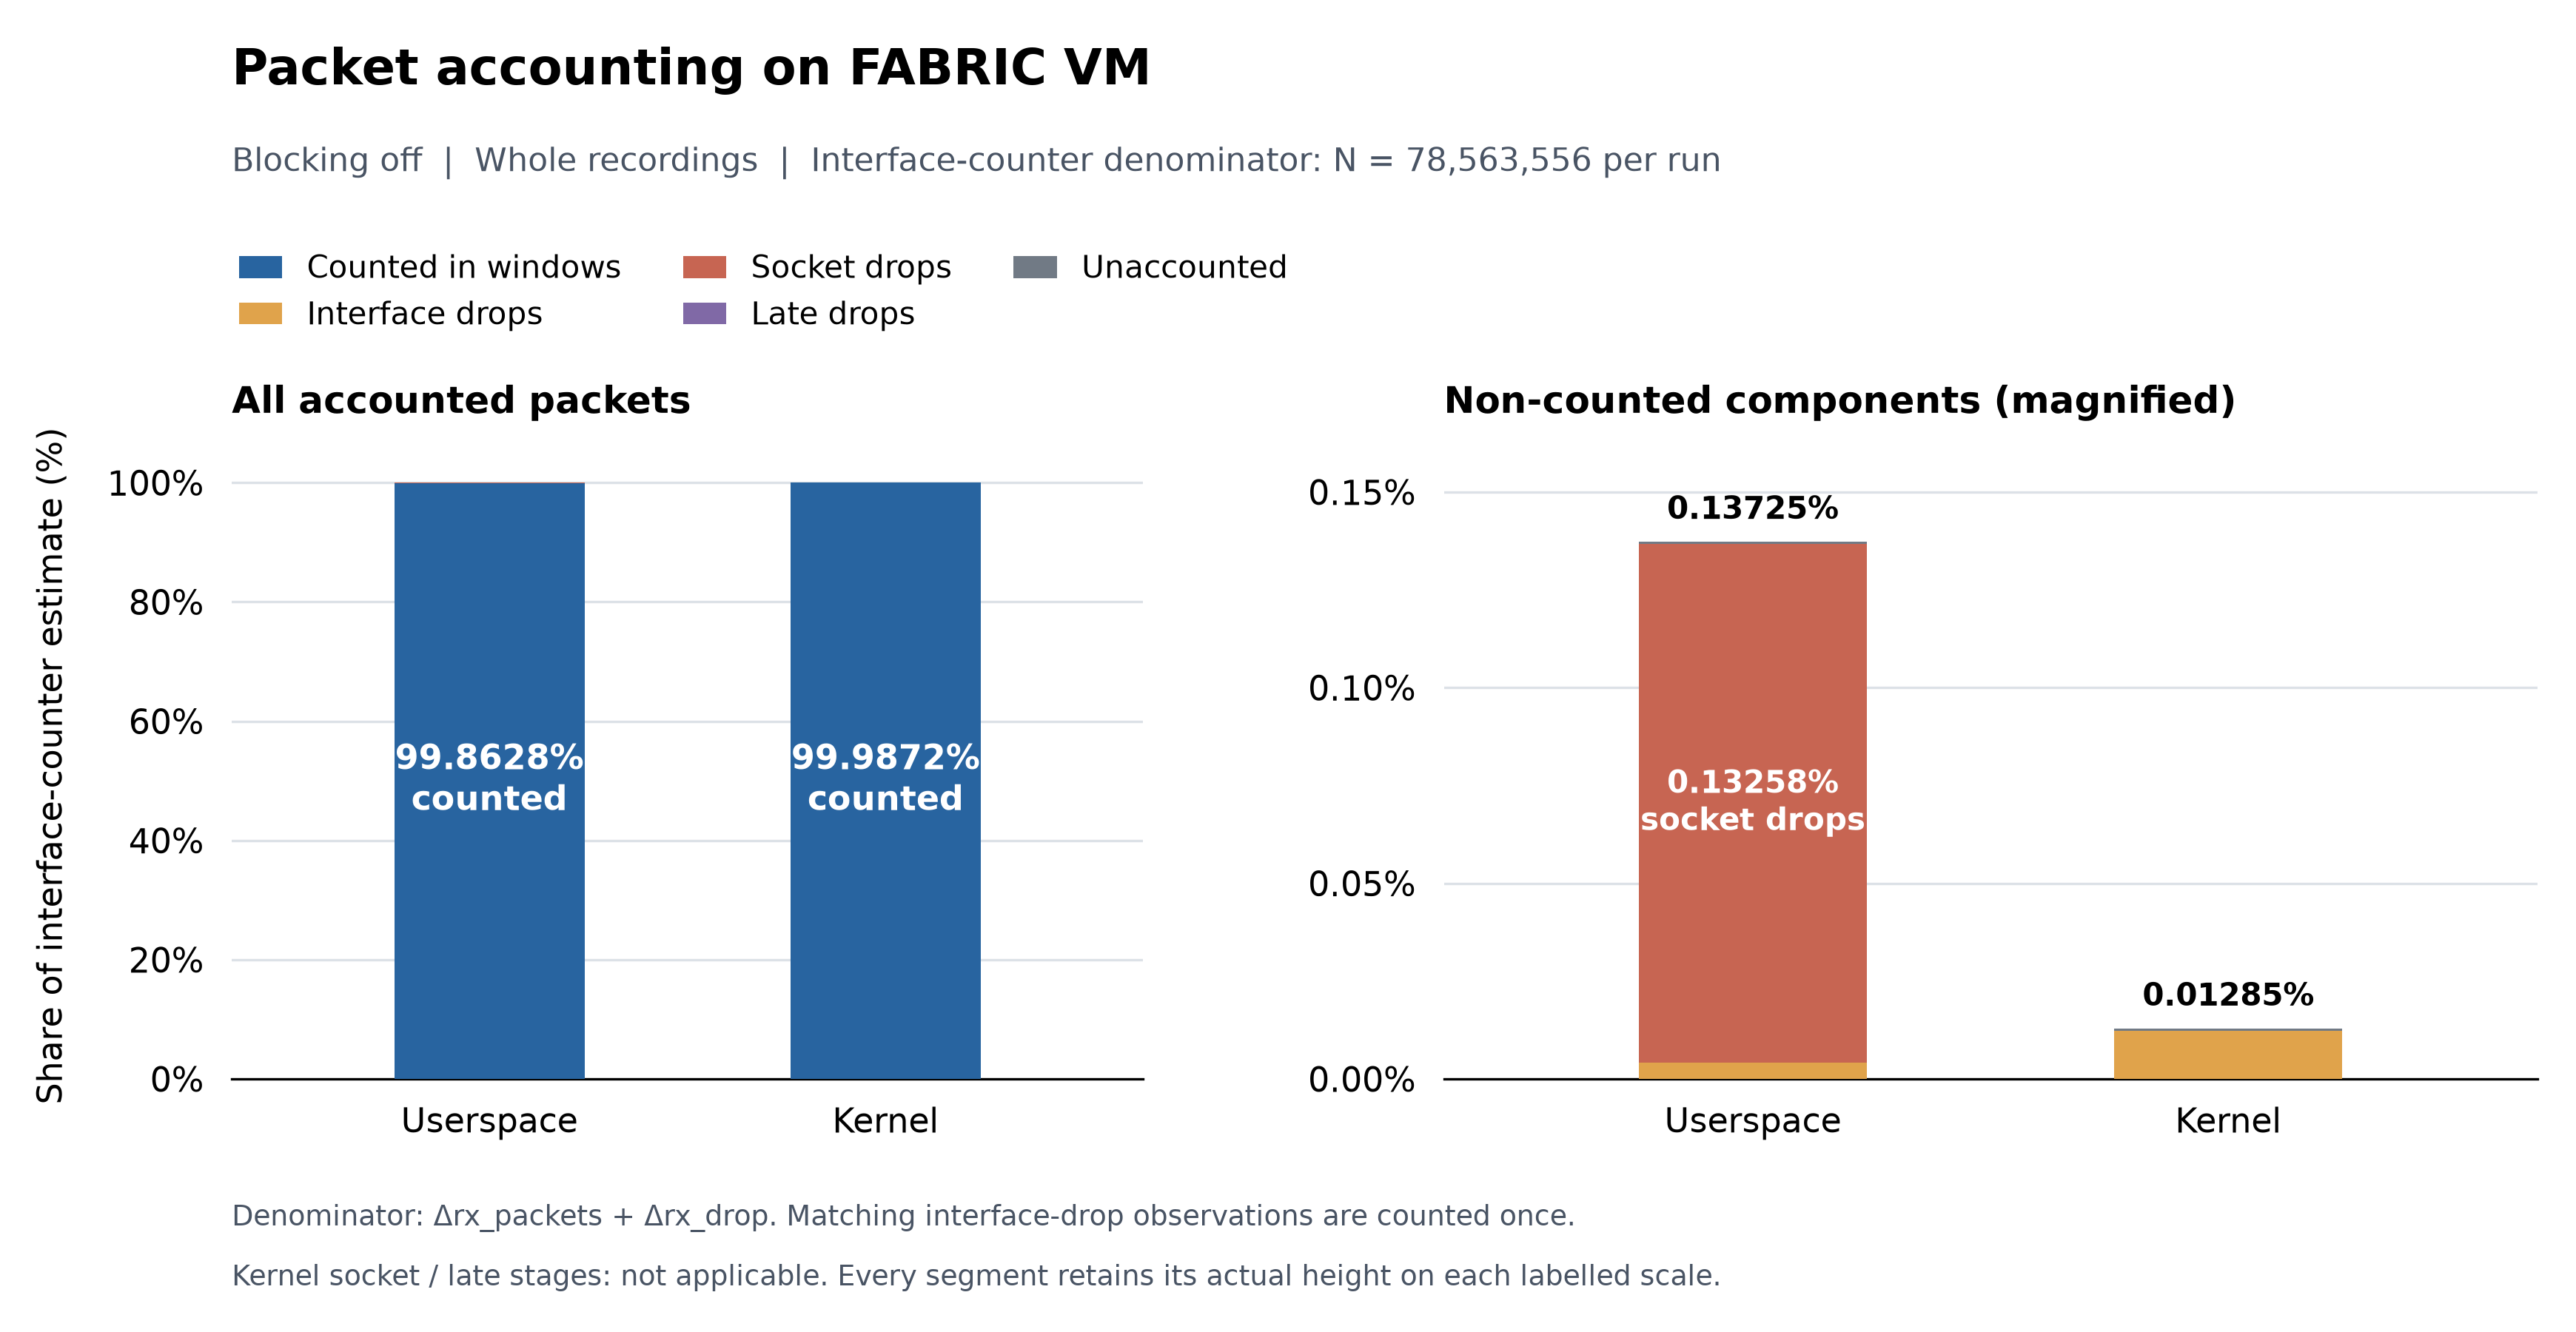
\includegraphics[width=\linewidth]{resources/testing-figures/fabric/figure-09-packet-accounting.png}
  \caption{Packet accounting on the FABRIC VM with blocking disabled. Shares use the whole-run interface-counter estimate; right: magnified non-counted components.}
  \label{fig:fabric-loss}
\end{figure}
\begin{table}[H]
  \centering
  \footnotesize
  \setlength{\tabcolsep}{4pt}
  \begin{tabular}{@{}lrrrr@{}}
    \toprule
    & \multicolumn{2}{c}{Userspace} & \multicolumn{2}{c}{Kernel} \\
    \cmidrule(lr){2-3}\cmidrule(lr){4-5}
    & Packets & \% & Packets & \% \\
    \midrule
    Interface-counter estimate & 78,563,556 & 100.000 & 78,563,556 & 100.000 \\
    Interface drops (\texttt{rx\_drop}) & 3,251 & 0.00414 & 9,689 & 0.01233 \\
    Capture-socket drops & 104,156 & 0.13258 & -- & -- \\
    Late drops & 13 & 0.000017 & -- & -- \\
    Unaccounted / other & 405 & 0.000516 & 405 & 0.000516 \\
    Counted in windows & 78,455,731 & 99.86275 & 78,553,462 & 99.98715 \\
    \bottomrule
  \end{tabular}
  \caption{Whole-run packet accounting on the FABRIC VM, blocking disabled.
  The denominator is $\Delta\mathrm{rx\_packets}+\Delta\mathrm{rx\_drop}$,
  an interface-counter estimate rather than an independently verified wire
  total. Identical observations of interface loss in \texttt{rx\_drop} and
  \texttt{rx\_out\_of\_buffer} are counted once.}
  \label{tab:fabric-loss}
\end{table}

Both FABRIC implementations count almost the entire interface-counter
estimate: 99.86275\% for userspace and 99.98715\% for the kernel run
(Figure~\ref{fig:fabric-loss}, Table~\ref{tab:fabric-loss}). The userspace
run records 104,156 socket drops and 13 late drops; the kernel path has
neither of these userspace capture stages. Interface drops are higher in
the kernel recording, 9,689 versus 3,251, but its counted total is still
97,731 packets larger. This is a much smaller difference than on the Pi.

The residual is 405 packets in each run. In userspace it is exactly the
number of parser-skipped frames; the kernel residual is retained without
assigning a loss cause. The saved evaluator reports window-loss estimates
of 0.87\% and 0.75\%, respectively, over windows fully inside the mapped
excerpt. These are alignment-dependent estimates, distinct from the
whole-run counter balance and from the 75-window scoring exclusion.


% ---------------------------------------------------------------------
\subsection{CPU Utilisation}
\label{sec:res-cpu}

\paragraph{Raspberry Pi 400}

\begin{figure}[H]
  \centering
  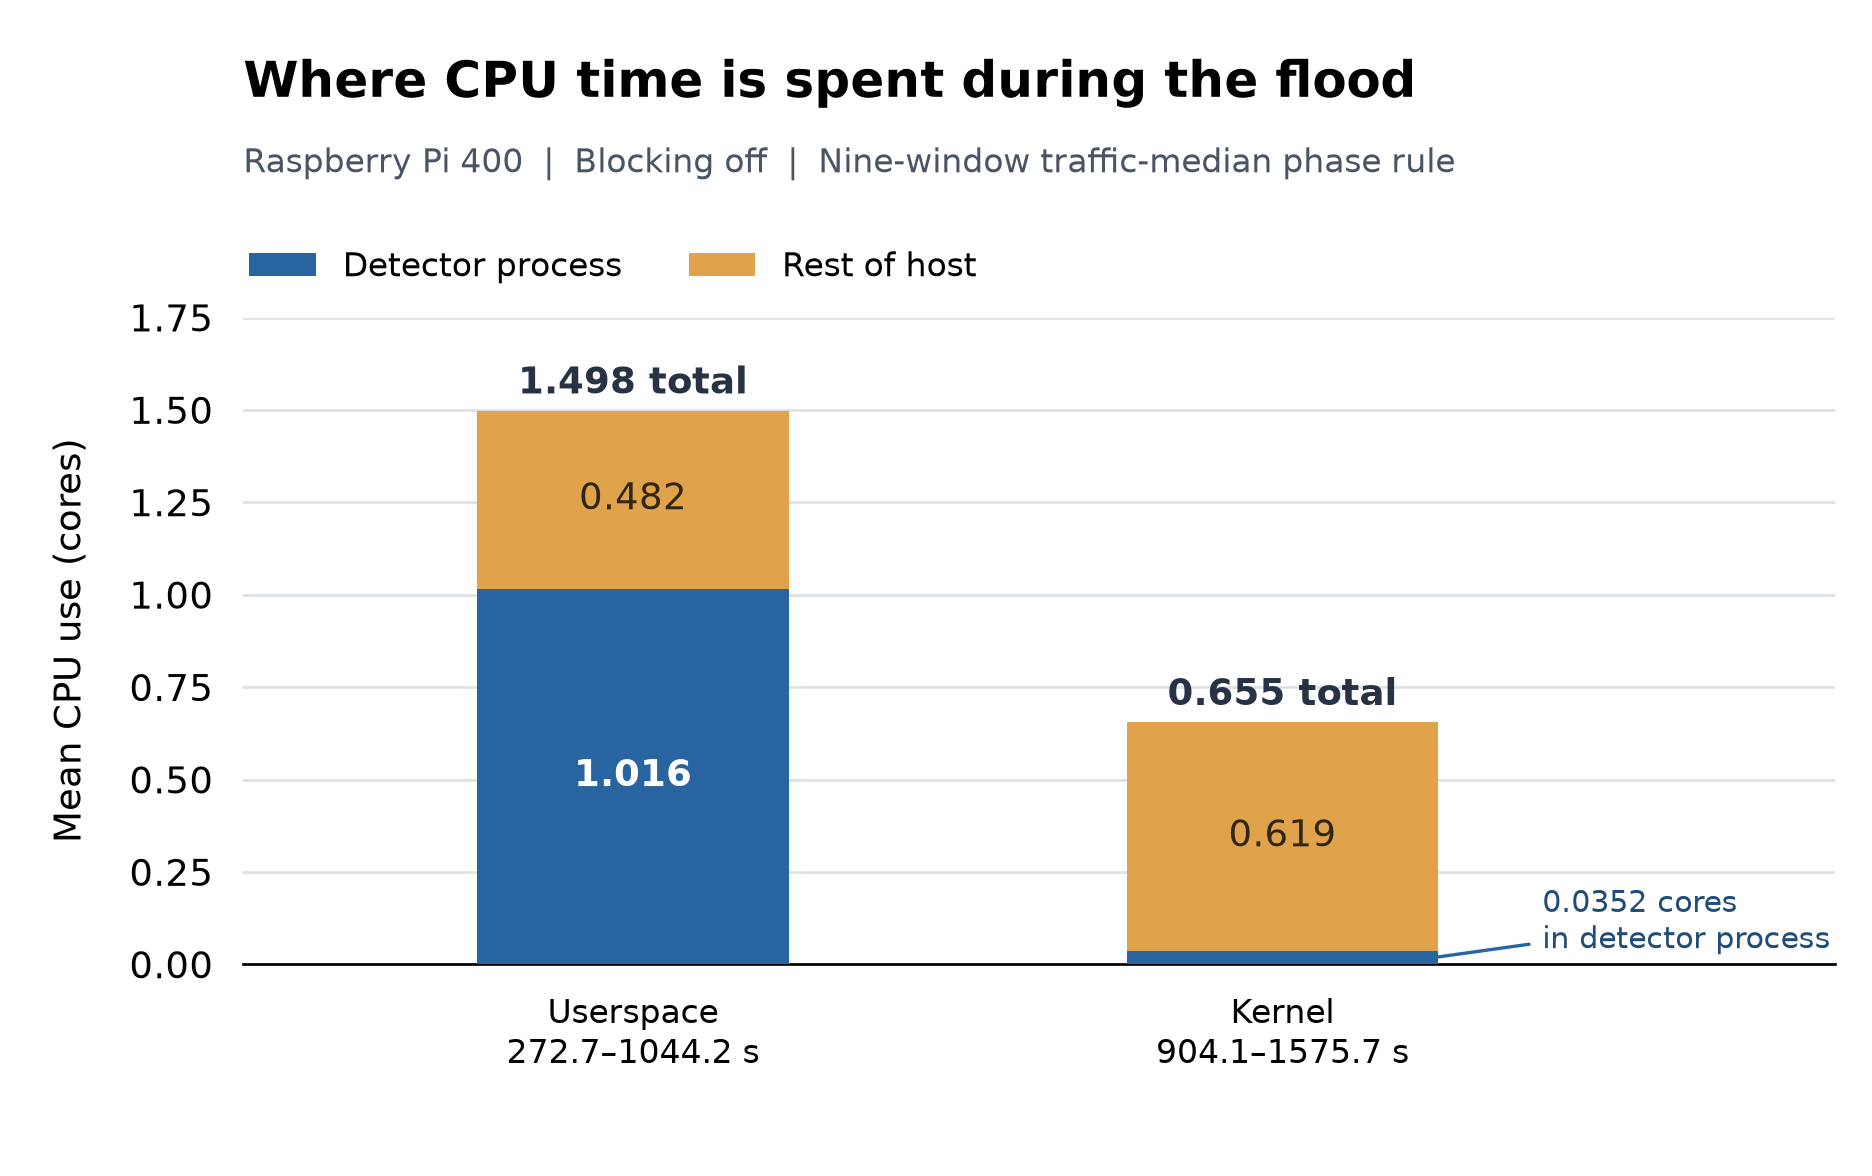
\includegraphics[width=\linewidth]{resources/testing-figures/figure-10-cpu-breakdown.png}
  \caption{CPU breakdown on the Raspberry Pi 400 with blocking disabled, over the counted-flood intervals used in Table~\ref{tab:cpu}. Values are mean cores, split into detector process and rest of host, including software-interrupt time.}
  \label{fig:cpu-host}
\end{figure}

On the Raspberry Pi, the flood interval of each run is the span of windows identified in
Section~\ref{sec:res-workload}: 272.7--1044.2~s after the first recorded window for
userspace and 904.1--1575.7~s for the kernel implementation.

\begin{table}[H]
  \centering
  \small
  \begin{tabular}{lrr}
    \toprule
    & Userspace & Kernel \\
    \midrule
    Host CPU, whole run (\% of all cores)       & 13.44 & 6.65 \\
    Host CPU, flood (\% of all cores)           & 38.7  & 16.5 \\
    Detector process, flood (\% of one core)    & 101.6 & 3.5 \\
    Counted rate, flood mean (kpps)             & 24.3  & 104.9 \\
    Counted rate, flood maximum window (kpps)   & 50.6  & 219.3 \\
    Host CPU time per counted packet, flood ($\mu$s) & 61.7 & 6.2 \\
    \bottomrule
  \end{tabular}
  \caption{CPU utilisation and counted packet rate with blocking disabled,
  Raspberry Pi 400. Host CPU time per counted packet is the whole-host CPU
  time during the flood divided by the packets counted in windows during
  the flood. It includes other host work and work on packets that were
  later dropped.}
  \label{tab:cpu}
\end{table}

During the flood, host CPU utilisation is 38.7\% for userspace and 16.5\%
for the kernel implementation, while the kernel implementation counts 4.3
times as many packets per second (Table~\ref{tab:cpu}). Whole-host CPU time
per counted packet is therefore 61.7 versus 6.2~$\mu$s. The userspace
detector process uses 101.6\% of one core during the flood, the kernel
detector process 3.5\%.

\paragraph{FABRIC VM}

\begin{figure}[H]
  \centering
  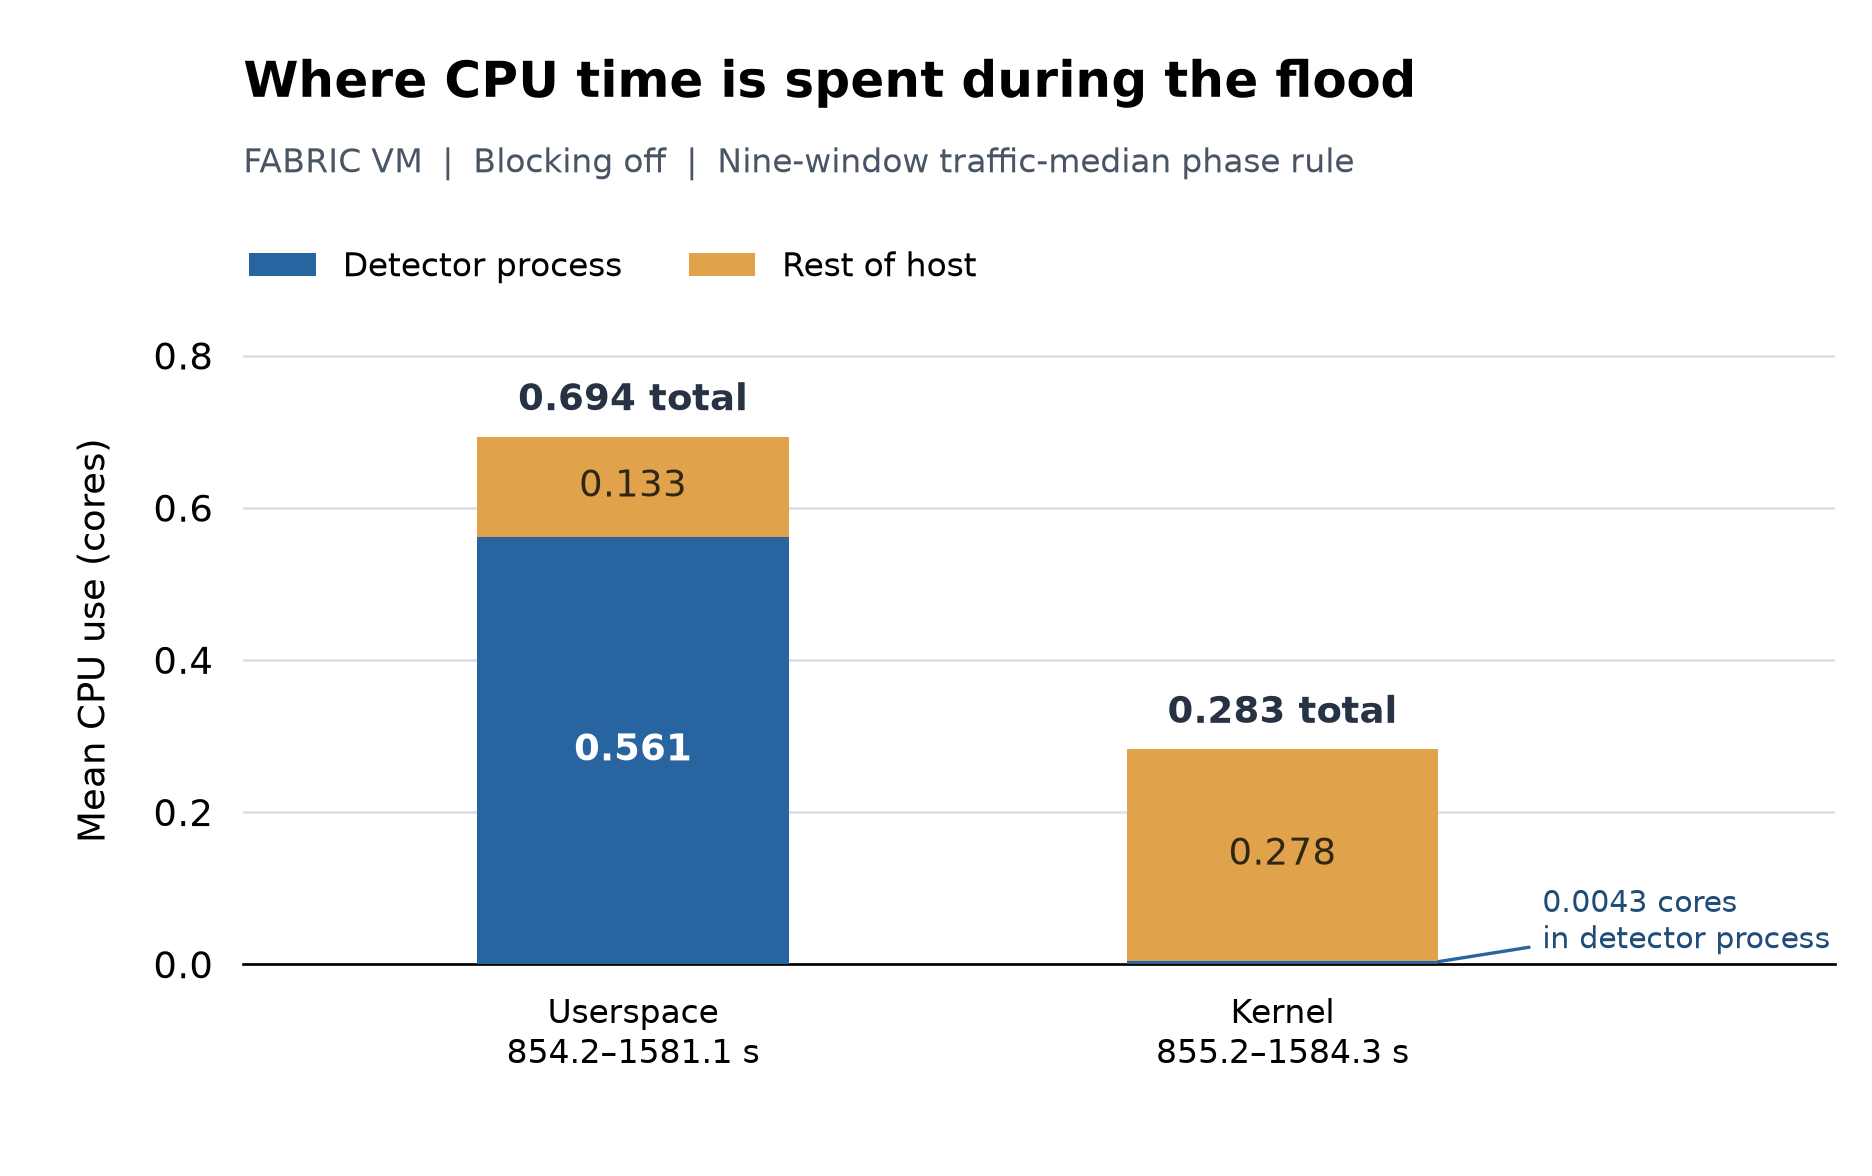
\includegraphics[width=\linewidth]{resources/testing-figures/fabric/figure-10-cpu-breakdown.png}
  \caption{CPU time during each FABRIC run's counted flood, blocking disabled. The stacks show mean cores in the detector process and the rest of the host; the latter includes unrelated work and kernel packet processing.}
  \label{fig:fabric-cpu}
\end{figure}

The FABRIC flood intervals are 854.2--1581.1~s for userspace and
855.2--1584.3~s for the kernel run, measured from the first recorded
window using the nine-window median rule above. Figure~\ref{fig:fabric-cpu}
uses these same intervals.

\begin{table}[H]
  \centering
  \small
  \begin{tabular}{@{}lrr@{}}
    \toprule
    & Userspace & Kernel \\
    \midrule
    Host CPU, whole run (\% of all cores) & 10.20 & 4.25 \\
    Host CPU, flood (\% of all cores) & 37.1 & 14.2 \\
    Detector process, flood (\% of one core) & 56.1 & 0.43 \\
    Counted rate, flood mean (kpps) & 103.6 & 103.4 \\
    Counted rate, maximum window (kpps) & 143.3 & 143.2 \\
    Host CPU time per counted packet ($\mu$s) & 6.69 & 2.73 \\
    \bottomrule
  \end{tabular}
  \caption{CPU utilisation and counted traffic on the FABRIC VM, blocking disabled. CPU percentages use ratios of summed contemporaneous counters. CPU time per counted packet includes all host work, including work on traffic subsequently dropped.}
  \label{tab:fabric-cpu}
\end{table}

During the flood, the counted rates are almost equal, 103.6 versus
103.4~kpps, while host utilisation is 37.1\% for userspace and 14.2\%
for the kernel implementation. Host CPU time per counted packet is
6.69 versus 2.73~$\mu$s (Table~\ref{tab:fabric-cpu}). The detector
process accounts for 56.1\% of one core in userspace and 0.43\% in
the kernel run. XDP's per-packet work is outside that process and remains
part of host CPU. Without a same-traffic no-detector baseline these
measurements do not isolate detector-only overhead.


% ---------------------------------------------------------------------
\subsection{Detection Quality}
\label{sec:res-detection}

Detection quality is scored against window-level ground truth derived from
the corrected flow labels, excluding the first 75 evaluated windows as
warm-up.

\paragraph{Raspberry Pi 400}

Table~\ref{tab:detection} reports the userspace run under the
evaluator's alignment and, as a preliminary sensitivity check, shifted by
295 windows (158~s) so that its flood onset matches the kernel run. The
shift is derived from counted traffic, not from verdicts. Because the
flood durations differ (Table~\ref{tab:coverage}), no single shift aligns
the whole userspace run.

% Onset-aligned column is preliminary until usr-acc-gen is re-run.
\begin{table}[H]
  \centering
  \small
  \begin{tabular}{lrrr}
    \toprule
    & \multicolumn{2}{c}{Userspace} & Kernel \\
    \cmidrule(lr){2-3}
    & Evaluator & Onset-aligned & Evaluator \\
    \midrule
    Attack-labelled windows  & 2,882 & 2,882 & 2,882 \\
    Benign-labelled windows  & 724   & 429   & 1,511 \\
    \midrule
    True positives (TP)      & 2,206 & 2,192 & 2,576 \\
    False positives (FP)     & 237   & 9     & 31 \\
    True negatives (TN)      & 487   & 420   & 1,480 \\
    False negatives (FN)     & 676   & 690   & 306 \\
    \midrule
    Recall (\%)              & 76.5  & 76.1  & 89.4 \\
    Precision (\%)           & 90.3  & 99.6  & 98.8 \\
    False-positive rate (\%) & 32.7  & 2.1   & 2.1 \\
    F1 score                 & 0.829 & 0.863 & 0.939 \\
    Accuracy (\%)            & 74.7  & 78.9  & 92.3 \\
    \bottomrule
  \end{tabular}
  \caption{Window-level detection quality, Raspberry Pi 400, blocking
  disabled. The onset-aligned column is preliminary.}
  \label{tab:detection}
\end{table}

\begin{table}[H]
  \centering
  \small
  \begin{tabular}{lrr}
    \toprule
    & Userspace & Kernel \\
    \midrule
    Before the flood: windows / flagged       & 432 / 2.8\%   & 1,515 / 2.2\% \\
    Flood: windows / flagged                  & 1,437 / 86.4\% & 1,251 / 97.3\% \\
    Low-rate tail: windows / flagged          & 1,736 / 68.4\% & 1,626 / 83.3\% \\
    \midrule
    Flood windows not flagged                 & 195 & 34 \\
    \quad with no packets in the two-window span & 183 & 32 \\
    \bottomrule
  \end{tabular}
  \caption{Share of scored windows flagged in each phase, Raspberry Pi 400,
  with phases taken
  from each run's own counted traffic. The phase split does not depend on
  the alignment to trace time.}
  \label{tab:phases}
\end{table}

\begin{figure}[H]
  \centering
  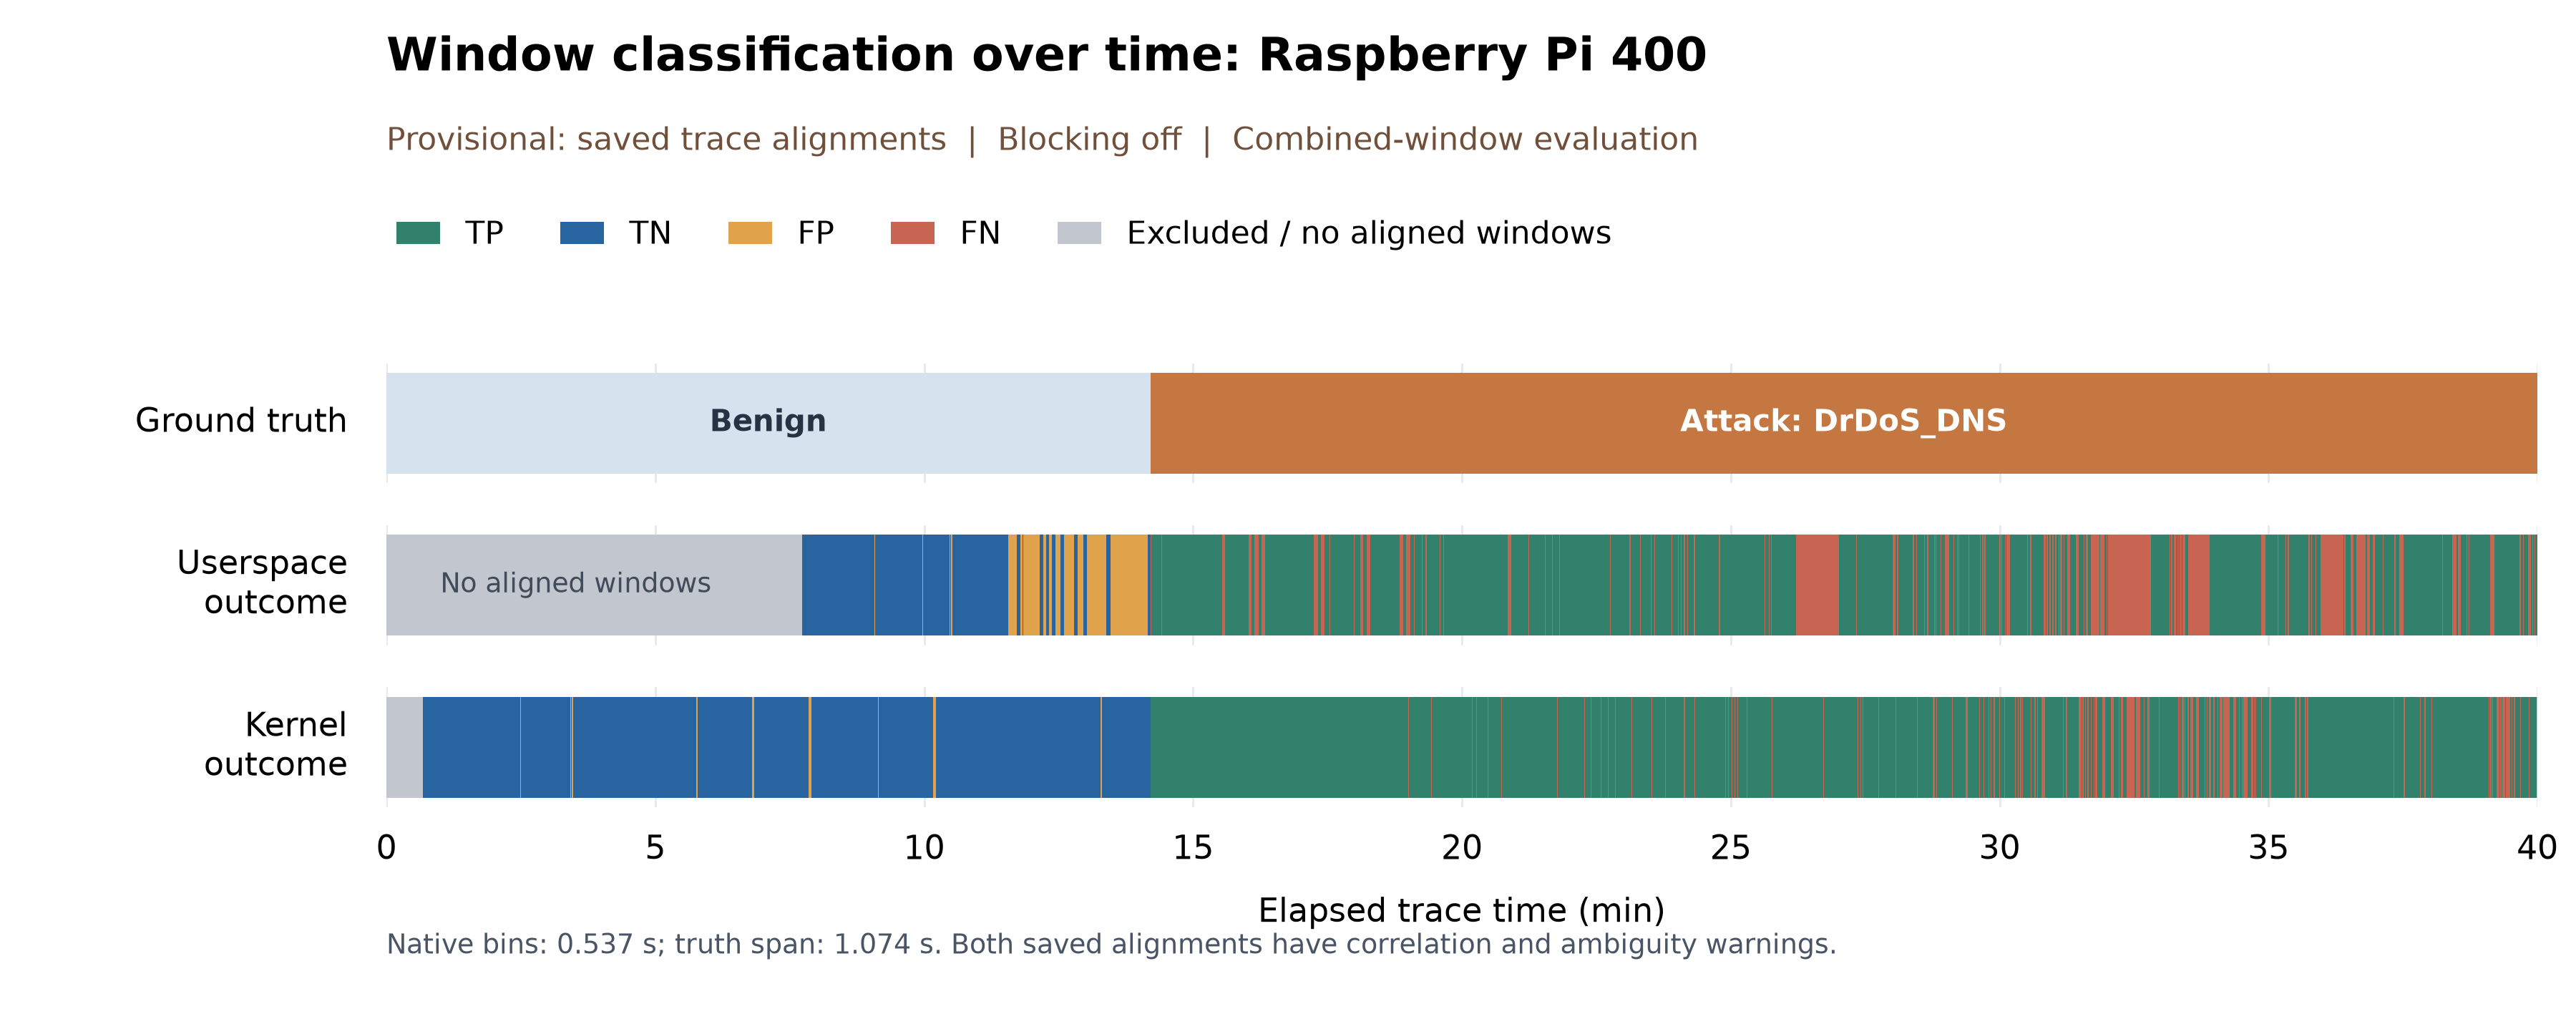
\includegraphics[width=\linewidth]{resources/testing-figures/figure-11-window-classification.png}
  \caption{Window classification over time, Raspberry Pi 400.}
  \label{fig:outcomes}
\end{figure}

Under the evaluator's alignment, 225 of the 237 userspace false positives
fall in the 156.8~s between its flood onset and the labelled attack start.
With the onset-aligned shift, the false-positive rate is 2.1\% for both
implementations, while recall remains lower for userspace: 76.1 versus
89.4\% (Table~\ref{tab:detection}). Before the flood, both implementations
flag 2--3\% of the windows. During the flood, 86.4\% of the userspace
windows are flagged against 97.3\% for the kernel implementation, and 183 of
the 195 unflagged userspace flood windows contain no packets over the whole
two-window span (Table~\ref{tab:phases}). Both implementations flag the
first window of the flood. \fillin{Low-rate tail. Comparison with Koshovyi
and Wu (precision $\approx$1.0, recall $\approx$0.40).}

\paragraph{FABRIC VM}

\begin{table}[H]
  \centering
  \small
  \begin{tabular}{@{}lrr@{}}
    \toprule
    & Userspace & Kernel \\
    \midrule
    Attack-labelled windows & 2,881 & 2,881 \\
    Benign-labelled windows & 1,512 & 1,512 \\
    True positives (TP) & 2,657 & 2,647 \\
    False positives (FP) & 33 & 37 \\
    True negatives (TN) & 1,479 & 1,475 \\
    False negatives (FN) & 224 & 234 \\
    Recall (\%) & 92.2 & 91.9 \\
    Precision (\%) & 98.8 & 98.6 \\
    False-positive rate (\%) & 2.2 & 2.4 \\
    F1 score & 0.954 & 0.951 \\
    Accuracy (\%) & 94.1 & 93.8 \\
    \bottomrule
  \end{tabular}
  \caption{Saved window-level detection quality on the FABRIC VM, blocking disabled. Both columns retain the evaluator alignment and are provisional because its alignment criteria fail.}
  \label{tab:fabric-detection}
\end{table}
\begin{table}[H]
  \centering
  \small
  \begin{tabular}{@{}lrr@{}}
    \toprule
    & Userspace & Kernel \\
    \midrule
    Before flood: windows / flagged & 1,512 / 2.2\% & 1,508 / 2.2\% \\
    Flood: windows / flagged & 1,354 / 99.9\% & 1,358 / 99.9\% \\
    Low-rate tail: windows / flagged & 1,527 / 85.4\% & 1,527 / 84.8\% \\
    Flood windows not flagged & 1 & 2 \\
    \quad with an empty two-window span & 1 & 2 \\
    \bottomrule
  \end{tabular}
  \caption{FABRIC scored-window flag rates by each recording's own traffic phase. The three half-open phase populations partition all 4,393 scored windows per run.}
  \label{tab:fabric-phases}
\end{table}
\begin{figure}[H]
  \centering
  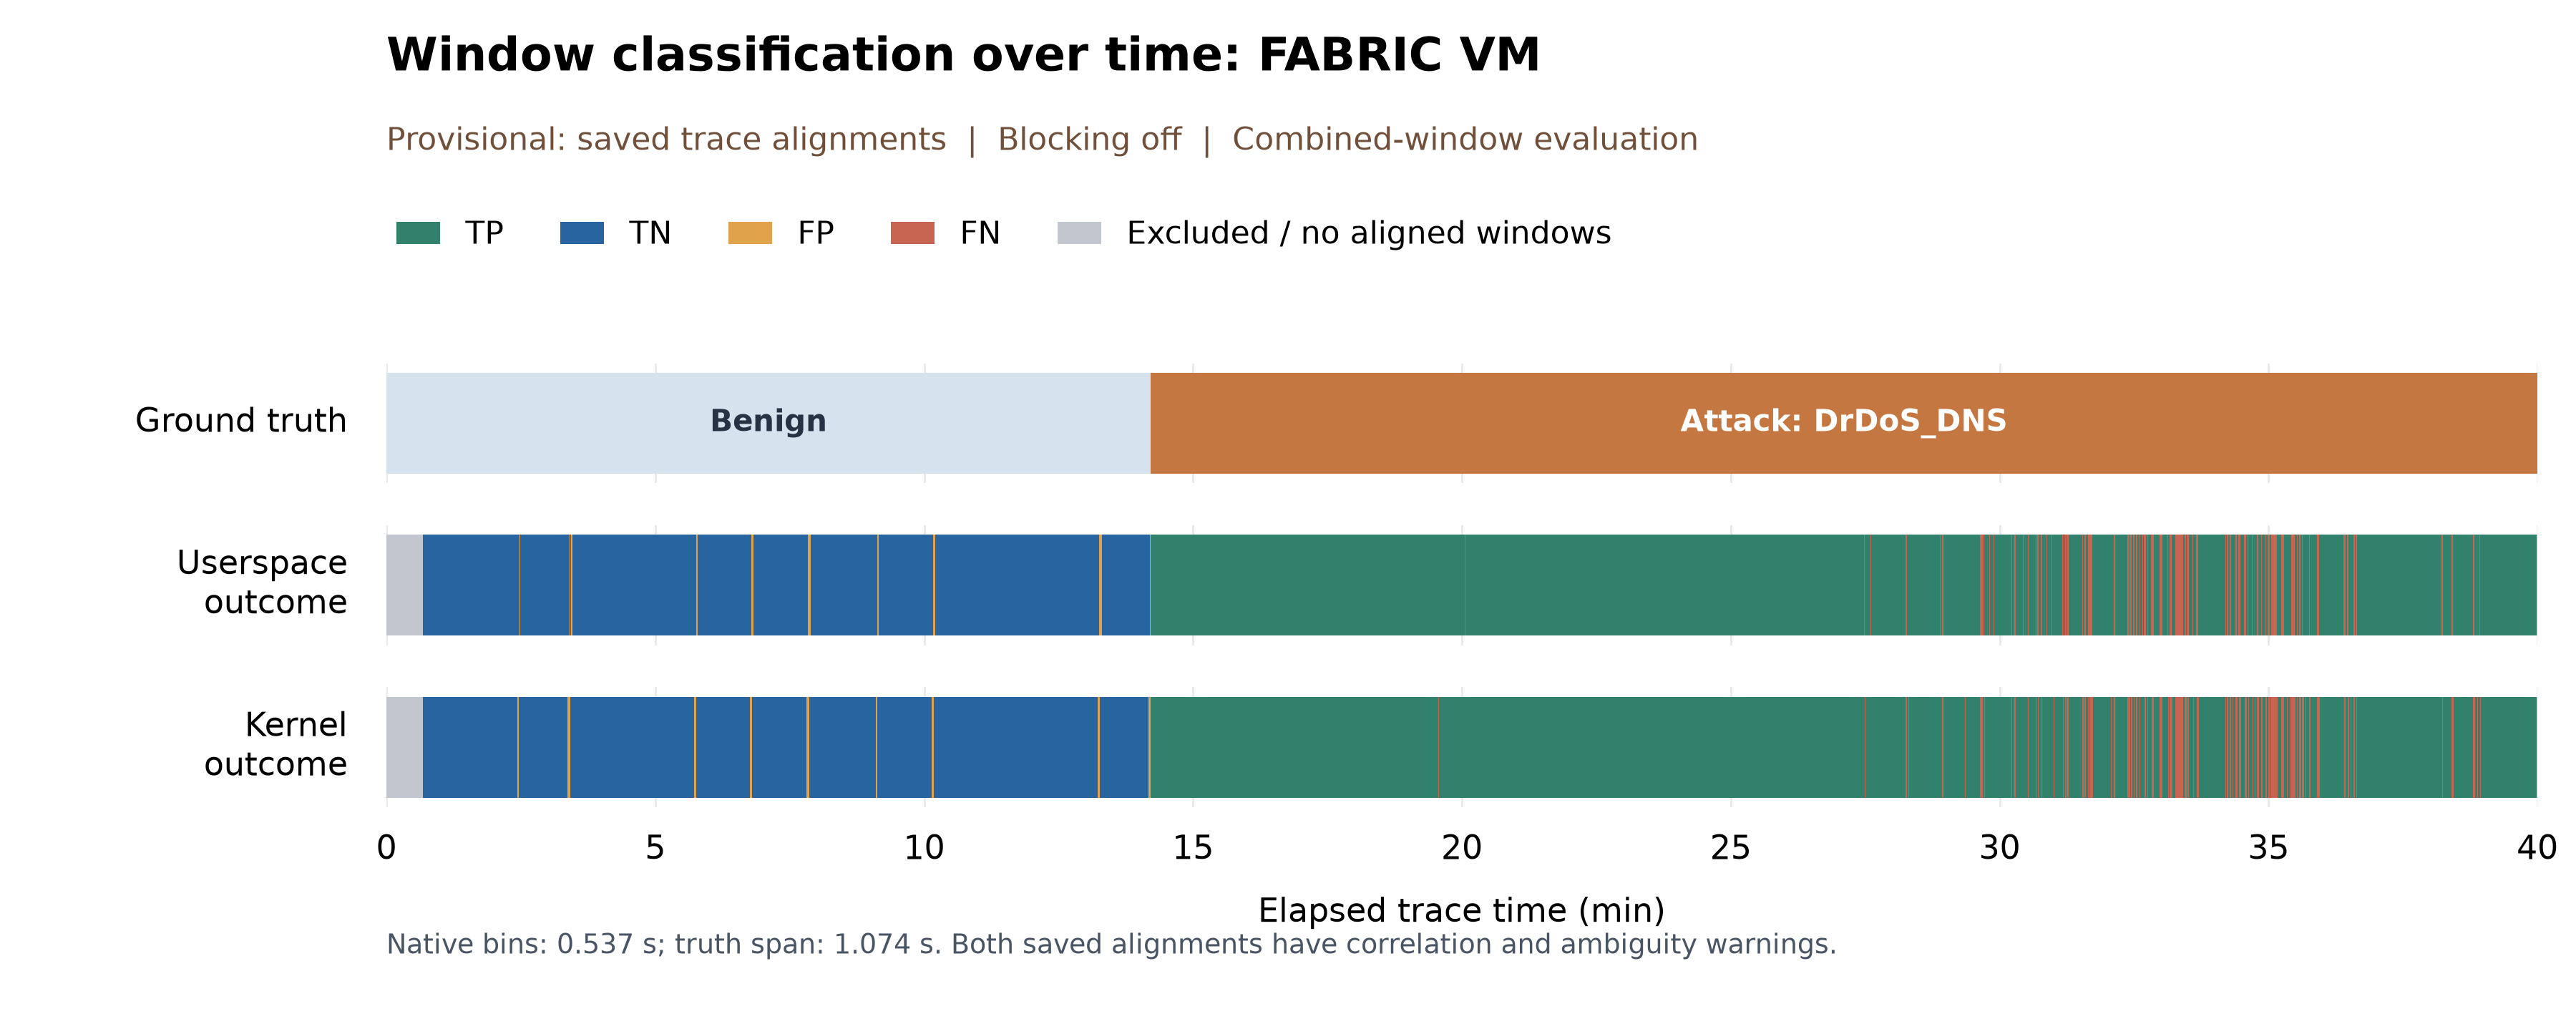
\includegraphics[width=\linewidth]{resources/testing-figures/fabric/figure-11-window-classification.png}
  \caption{Provisional window classification over time on the FABRIC VM. Grey marks excluded windows. The shared trace clock uses saved offsets; both alignments retain correlation and peak-ambiguity warnings.}
  \label{fig:fabric-outcomes}
\end{figure}

Under the saved alignments, the two FABRIC implementations have similar
observed detection quality: recall is 92.2\% versus 91.9\%, precision
98.8\% versus 98.6\%, and F1 0.954 versus 0.951 for userspace and kernel,
respectively (Table~\ref{tab:fabric-detection}). These small differences do
not establish an implementation advantage or statistical equivalence.

Both implementations flag the first window of their counted flood and
approximately 99.9\% of scored flood windows. The one unflagged userspace
flood window and two unflagged kernel flood windows have empty two-window
spans. Most false negatives occur in the low-rate tail: 223 of 224 for
userspace and 232 of 234 for the kernel implementation. Tail flag rates are
85.4\% and 84.8\% (Table~\ref{tab:fabric-phases}). Figure~\ref{fig:fabric-outcomes}
shows these windows on the saved trace mappings; the unresolved replay
timing prevents treating this as a validated temporal comparison.


% ---------------------------------------------------------------------
\subsection{Blocking Enabled}
\label{sec:res-blocking}

\paragraph{Raspberry Pi 400}

\begin{table}[H]
  \centering
  \small
  \begin{tabular}{lrr}
    \toprule
    & Userspace & Kernel \\
    \midrule
    Intentionally blocked in XDP (\%)  & 98.1 & 98.1 \\
    Passed XDP (\%)                    & 0.90 & 0.95 \\
    Interface drops (\%)               & 1.02 & 0.97 \\
    \midrule
    Block events                       & 49   & 49 \\
    Unique sources blocked             & 7    & 7 \\
    \quad of which attack sources      & \fillin{} & \fillin{} \\
    Windows flagged                    & 154  & 153 \\
    \midrule
    Host CPU, whole run (\% of all cores) & 5.68 & 5.85 \\
    Host CPU, flood (\% of all cores)     & 10.1 & 10.4 \\
    \bottomrule
  \end{tabular}
  \caption{Runs with blocking enabled (\texttt{usr-per-gen-1},
  \texttt{ker-per-gen-1}), Raspberry Pi 400. Percentages are of the packets
  seen by the interface. Blocklist entries expire after 60~s.}
  \label{tab:blocking}
\end{table}

On the Raspberry Pi with blocking enabled, XDP drops 98.1\% of the packets in both
implementations, and less than 1\% passes on to the detector. Interface
drops fall to approximately 1\%, and host CPU during the flood is 10.1\%
for userspace and 10.4\% for the kernel implementation
(Table~\ref{tab:blocking}). Both runs block the same 7 sources in 49 block
events. During the flood, traffic passes XDP in bursts approximately every
61~s, when blocklist entries expire before being renewed.

\paragraph{FABRIC VM}

\begin{table}[H]
  \centering
  \small
  \begin{tabular}{@{}lrr@{}}
    \toprule
    & Userspace & Kernel \\
    \midrule
    Intentionally blocked in XDP (\%) & 99.07 & 99.08 \\
    Passed XDP (\%) & 0.919 & 0.913 \\
    Interface drops (\%) & 0.00982 & 0.00571 \\
    New block events & 47 & 46 \\
    Refreshes of active entries & 23 & 29 \\
    Unique sources blocked & 7 & 6 \\
    \quad verified attack sources & -- & -- \\
    Windows flagged & 139 & 155 \\
    Host CPU, whole run (\% of all cores) & 0.52 & 0.57 \\
    Host CPU, flood (\% of all cores) & 1.52 & 1.32 \\
    \bottomrule
  \end{tabular}
  \caption{Blocking-enabled FABRIC runs, \texttt{usr-per-gen-1} and \texttt{ker-per-gen-1}. Percentages use the whole-run interface-counter estimate. New block events exclude refreshes. Per-source attack identity cannot be verified without the corrected flow-label file.}
  \label{tab:fabric-blocking}
\end{table}

With blocking enabled, XDP intentionally drops 99.07\% of the interface-counter
estimate for userspace and 99.08\% for the kernel run. Approximately 0.92\%
passes XDP, including traffic subsequently lost at the capture socket or
excluded by the parser. Interface drops account for 0.00982\% and 0.00571\%,
respectively (Table~\ref{tab:fabric-blocking}).

Userspace records 47 new block events affecting seven distinct sources and
23 refreshes; the kernel run records 46 new events affecting six sources
and 29 refreshes. Thus the successful per-IP update totals are 70 and 75.
Both manifests record a 60~s expiry and no blocklist errors. The source
counts describe successful updates, not verified malicious-source counts.

The flood is located from counted plus intentionally blocked packets,
with recorded socket drops added for userspace. Its intervals are
853.6--1581.6~s and 855.2--1583.2~s on the local first-window clocks.
Host utilisation during those intervals is 1.52\% and 1.32\%, versus
37.1\% and 14.2\% in the blocking-disabled runs. This workload suppresses
almost all post-XDP traffic; it does not measure full-stream counting
capacity. Both recordings end as interrupted after approximately 44.5
minutes, with recorded window/block totals retained over the observed run.


% ---------------------------------------------------------------------
\subsection{Memory and Decision Delay}
\label{sec:res-other}

\paragraph{Raspberry Pi 400}

\begin{table}[H]
  \centering
  \small
  \begin{tabular}{lrr}
    \toprule
    & Userspace & Kernel \\
    \midrule
    Cgroup main memory, median (MiB)     & 7.32  & 7.20 \\
    Separately charged BPF maps (KiB)    & 150.3 & 283.1 \\
    Main + BPF maps (MiB)                & 7.47  & 7.47 \\
    \midrule
    Window end to verdict, median / p95 (ms) & 10.75 / 11.72 & 12.17 / 13.65 \\
    Verdict computation, median / p95 (ms)   & 0.21 / 0.76   & 0.89 / 2.05 \\
    \bottomrule
  \end{tabular}
  \caption{Memory (blocking enabled) and decision delay (blocking disabled),
  Raspberry Pi 400.}
  \label{tab:other}
\end{table}

On the Raspberry Pi, including the BPF maps, both implementations use 7.47~MiB
(Table~\ref{tab:other}). The kernel implementation's median time from window
end to verdict is 1.4~ms longer, of which 0.7~ms is longer verdict
computation, which in the kernel implementation includes reading the
per-IP counts from the BPF maps. Both delays are below
14~ms at the 95th percentile, against a window length of 537~ms.

\paragraph{FABRIC VM}

\begin{table}[H]
  \centering
  \small
  \begin{tabular}{@{}lrr@{}}
    \toprule
    & Userspace & Kernel \\
    \midrule
    Cgroup main memory, median (MiB) & 7.09 & 7.01 \\
    Separately charged BPF maps (KiB) & 119.0 & 251.6 \\
    Main + BPF maps (MiB) & 7.20 & 7.26 \\
    Window end to verdict, median / p95 (ms) & 10.22 / 11.13 & 10.82 / 11.39 \\
    Verdict computation, median / p95 (ms) & 0.14 / 0.27 & 0.20 / 0.43 \\
    \bottomrule
  \end{tabular}
  \caption{FABRIC memory with blocking enabled and local decision timing with blocking disabled. Memory medians are sample-based; separately charged maps are added once. Timing uses evaluated windows with detector \texttt{warm\_up=false}, distinct from the 75-window scoring mask.}
  \label{tab:fabric-other}
\end{table}

Including the recorded BPF maps, median memory is 7.20~MiB for userspace and
7.26~MiB for the kernel implementation (Table~\ref{tab:fabric-other}). Main
memory alone is slightly smaller in the kernel run, but its separately
charged maps are larger: 251.6 versus 119.0~KiB. Program/JIT memory is not
included in these totals.

The kernel implementation's median time from window end to verdict is
10.82~ms, compared with 10.22~ms for userspace; verdict computation is
0.20 versus 0.14~ms. Both 95th-percentile decision delays are below 11.4~ms
against the 536.9~ms window length. These are local window-closing and
verdict-availability measurements, independent of trace-to-live alignment.
They do not measure attack-onset response, individual-packet execution time
or end-to-end application latency.


% ---------------------------------------------------------------------
\subsection{Summary}
\label{sec:res-summary}

\begin{table}[H]
  \centering
  \small
  \setlength{\tabcolsep}{4pt}
  \begin{tabular}{llll}
    \toprule
    & \multicolumn{2}{c}{Kernel vs.\ userspace} & \\
    \cmidrule(lr){2-3}
    Measure & Raspberry Pi 400 & FABRIC VM & Note \\
    \midrule
    Packets counted         & 73.6\,M vs.\ 21.1\,M  & 78.55\,M vs.\ 78.46\,M & whole run \\
    Host CPU, flood         & 16.5 vs.\ 38.7\%      & 14.2 vs.\ 37.1\% & own flood interval \\
    CPU per counted packet  & 6.2 vs.\ 61.7\,$\mu$s & 2.7 vs.\ 6.7\,$\mu$s & all host work \\
    Recall                  & 89.4 vs.\ 76.1\%      & 91.9 vs.\ 92.2\%$^{b}$ & preliminary$^{a}$ \\
    False-positive rate     & 2.1 vs.\ 2.1\%        & 2.4 vs.\ 2.2\%$^{b}$ & preliminary$^{a}$ \\
    Host CPU, blocking on   & 10.4 vs.\ 10.1\%      & 1.32 vs.\ 1.52\% & flood \\
    Memory incl.\ BPF maps  & 7.47 vs.\ 7.47\,MiB   & 7.26 vs.\ 7.20\,MiB & blocking on \\
    Window end to verdict   & 12.17 vs.\ 10.75\,ms  & 10.82 vs.\ 10.22\,ms & median \\
    \bottomrule
  \end{tabular}
  \caption{Key observed differences, one run per configuration, blocking
  disabled unless stated. $^{a}$Pi userspace onset-aligned. $^{b}$FABRIC uses the saved evaluator alignments; both remain provisional.}
  \label{tab:summary}
\end{table}

\fillin{RQ1 and RQ2 in two to three sentences each, separating the measured
resource results from the detection results that depend on alignment.}
